\documentclass[preprintnumbers,amsmath,amssymb,superscriptaddress,twocolumn,showpacs]{revtex4-1}
%\documentclass[preprintnumbers,amsmath,amssymb]{revtex4}
\usepackage{graphicx}% Include figure files
\usepackage{dcolumn}% Align table columns on decimal point
\usepackage{bm}% bold math
\usepackage{natbib}
\usepackage{physics}
\usepackage[caption=false]{subfig}

%\newcommand{|}{Y$_2$SiO$_5$}
\def\sgn{\mathop{\rm sgn}}
\newcommand{\be}{\begin{equation}}
\newcommand{\ee}{\end{equation}}
\newcommand{\bea}{\begin{eqnarray}}
\newcommand{\eea}{\end{eqnarray}}

\begin{document}

\title{TBA}

\author{C. Pellet-Mary$^1$, M. Perdriat$^1$, G. H\'etet} 

\affiliation{Laboratoire De Physique de l'\'Ecole Normale Sup\'erieure, \'Ecole Normale Sup\'erieure, PSL Research University, CNRS, Sorbonne Universit\'e, Universit\'e Paris Cit\'e , 24 rue Lhomond, 75231 Paris Cedex 05, France.}

\begin{abstract}
C'est trop bien
\end{abstract}

\maketitle
Blabla sur les NV, les ensembles etc.

In this letter/article, we characterize the depolarization of the spins observed for dense ensemble of NV centers in zero magnetic field and its potential application for DC magnetometry. While the main mechanism behind the depolarization, the lift in the degeneracy between the four classes of NV centers, is already well studied and can be exploited in a microwave-less vector magnetometry protocol, we found two other depolarization mechanisms specific to the zero-field region which could play an important role in the low-field magnetometry protocol.

The $T_1$ depolarization dynamics of single or sparse NV centers at room temperature is dominated by a two-phonon Raman process, which depends on the crystal lattice temperature but does not (?) depend on the external magnetic field. However, it has been observed that dense NV centers ensemble have an additional spin lifetime contribution which depends greatly on the magnetic field and not on the temperature. This effect has been attributed to cross-relaxation between the NV centers through dipole-dipole coupling. Some inhomogeneity between the NV centers is further needed in order to explain the depolarization of the spin ensemble.

The main signature of the spin depolarization in low field is the characteristic dip in photoluminescence (PL) observed only for high density ($\gtrsim 1$ ppm) of NV centers, as shown on fig [X]. The decrease in the spins' lifetime in zero field makes the optical polarization scheme of the NV centers less effective and therefore reduce the population of the bright $\ket{0}$ spin state. The reason for the decrease in PL at higher magnetic field values is the mixing of the bright spin state $\ket{0}$ to the darker state $\ket{-1}$ induced by the transverse magnetic field. This effect does not modify (on first approximation) the spins' lifetime, and is common to both dense and sparse samples.

The additional spin depolarization observed 

\begin{figure}
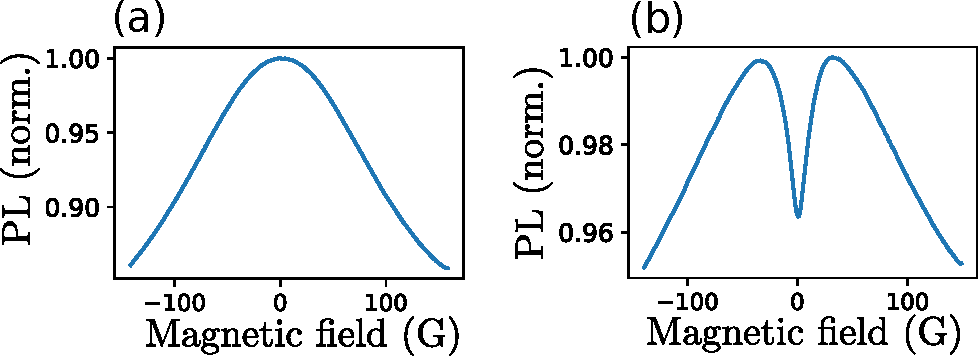
\includegraphics[width=0.45\textwidth]{Figures/fig dense vs pas dense}
\caption{Todo}
\label{PL_NV_density}
\end{figure}

\begin{figure}
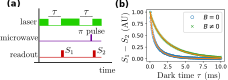
\includegraphics[width=0.45\textwidth]{Figures/fig T1}
\caption{Todo}
\label{T1}
\end{figure}

\begin{figure*}
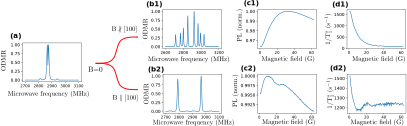
\includegraphics[width=.95\textwidth]{Figures/fig 100 vs 1x1x1x1}
\caption{Dependency of the magnetic field angle for the zero field depolarization. (a) ODMR spectrum in zero field. (b) ODMR spectrum for a magnetic field $\approx$ 60 G. The field is aligned (b2) or misaligned (b1, $\approx 24^\circ$ of misalignment) with the crystalline [100] direction. (c) Normalized photoluminescence of the NV$^-$ ensemble as a function of the magnetic field amplitude for the same field orientations as fig (b). (d) Stretch part of the lifetime decay as a function of the magnetic field amplitude for the same field orientations as fig (b).}
\label{100_VS_1x4}
\end{figure*}


\begin{figure}
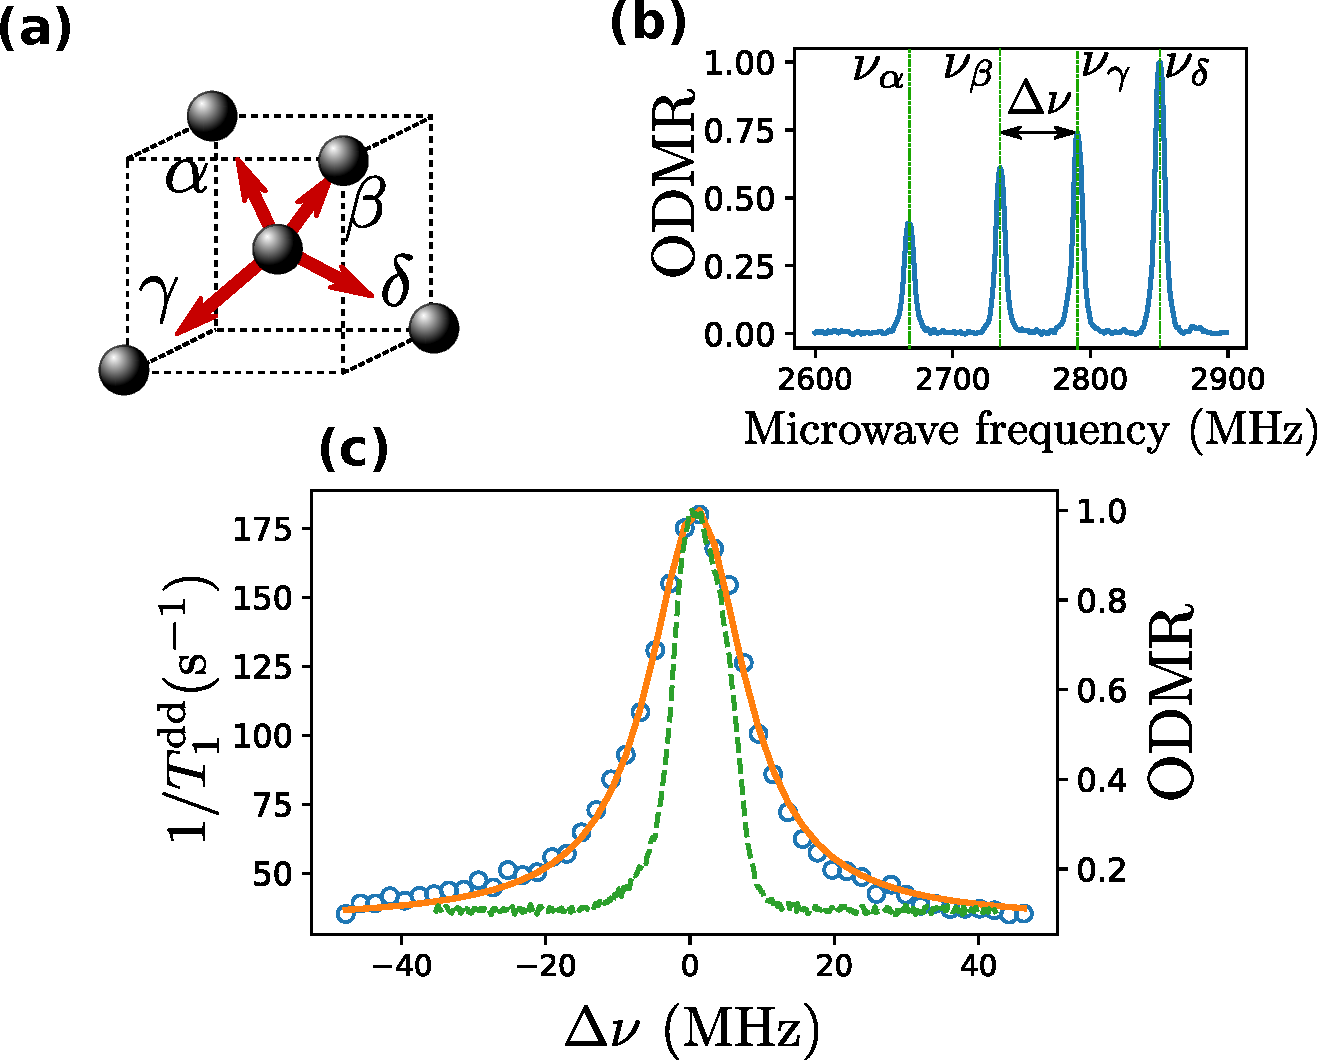
\includegraphics[width=0.45\textwidth]{Figures/fig largeur fluct}
\caption{Modification of the stretch lifetime for two near-resonant classes. (a) ODMR spectrum with amplitude modulation of the microwave for the $\ket{0} \to \ket{-1}$ transition of two separate NV classes. The frequency detuning between the two transitions is denoted $\Delta \nu$. (b) Stretch part of the lifetime decay for one of the two classes as function of the frequency detuning (blue circles), fitted by a Lorentzian with half width at half maximum 8.04 MHz . Green dashed line correspond to the ODMR width of a single class stretched by a factor $\sqrt 2$, approximating the overlap of the two classes (see SI).}
\label{largeur_fluct}
\end{figure}

\begin{figure}
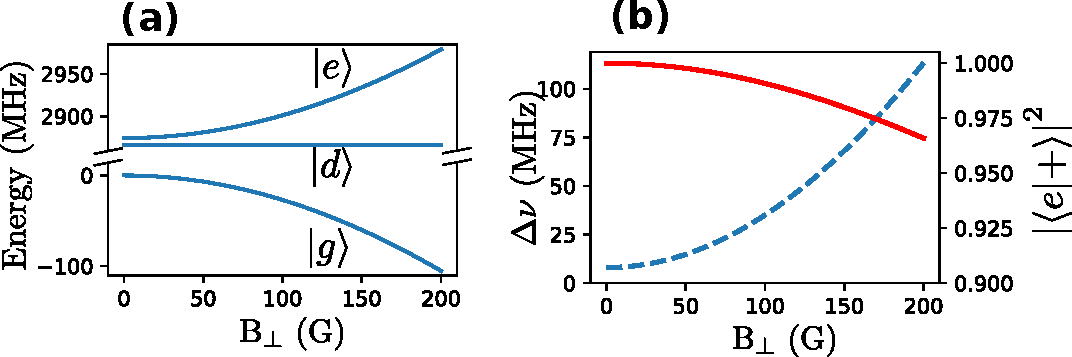
\includegraphics[width=0.45\textwidth]{Figures/fig transverse field simu}
\caption{Simulated eigenstates of the spin Hamiltonian in the presence of purely transverse magnetic field. (a) Energies of the three eigenstates $\ket{g}$, $\ket{d}$ and $\ket{e}$ as a function of the magnetic field amplitude. (b) Blue dashed curve : frequency detuning between the two transitions $\ket{g} \leftrightarrow \ket{d}$ and $\ket{g} \leftrightarrow \ket{e}$. Plain red curve : projection of $\ket{e}$ on $\ket{+}=(\ket{+1}+\ket{-1})/\sqrt{2}$ as a function the magnetic field. Is equal to the projection of $\ket{g}$ on $\ket{0}$.}
\label{calculs_B_transverse}
\end{figure}

\begin{figure}
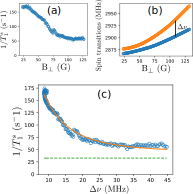
\includegraphics[width=0.45\textwidth]{Figures/fig transverse field}
\caption{Modification of the stretch lifetime in the presence of purely transverse magnetic field. (a) Stretch component of the ensemble lifetime as a function of the field amplitude. (b) Measured transition frequencies through ODMR spectrum. (c) Stretch component of the lifetime as a function of the frequency detuning between the two transistions (blue circles), fitted by a Lorentzian centered in $\Delta \nu=0$ with half width at half maximum 8MHz. The green dashed line correspond to the lifetime of a single class aligned with the magnetic field.}
\label{exp_B_transverse}
\end{figure}

\section*{acknowledgements}


\bibliography{CR}



\end{document}